% The format (A5) is selected to facilitate reading on small
% devices and should NOT be changed. 
\documentclass[a5paper,10pt,oneside]{article}

% The package babel is loaded for Swdish with Swedish hyphenation,
% replaces "Contents" with "Innehållsförteckning, "References"
% with "Litteraturförteckning", etc.
\usepackage[swedish]{babel}

\usepackage[T1]{fontenc}

% The package "inputenc" lets us specify what character encoding
% has been used to save the .tex file. If your computer runs
% Linux, the encoding is probably "utf8" by default, while under
% Windows the default will probably be "latin1" The wrong
% character encoding may give strange signs instead of "å", "ä"
% and "ö" or may result in compilation errors.

%\usepackage[latin1]{inputenc} % Probably right if you use Windows
\usepackage[utf8]{inputenc}  % Probably right if you use Linux

% The packages listed below are optional and can be removed if you
% don't use them 
\usepackage{graphicx} 
\usepackage{cite}
\usepackage{url}
\usepackage{ifthen}
\usepackage{listings}	


% These two lines set up options for the listings package and
% can be removed if you don't use it, or changed if you, e.g, 
% use another language than Java. 
% For more information about the listings package see:
% ftp://ftp.tex.ac.uk/tex-archive/macros/latex/contrib/listings/listings.pdf
\def \lstlistingname {Kodexempel}
\lstset{language=Java,tabsize=3,numbers=left,frame=L,floatplacement=hbtp}


\usepackage{ifpdf}
\ifpdf
	\usepackage[hidelinks]{hyperref}
\else
	\usepackage{url}
\fi


% Change NR and TITLE below to appropriate values
\title{Tema NR: 3 Träd}

% Write the name and user namn for all participants in the group here.
% Separate persons with \and
\author{Oscar Törnquist \url{osta3589} \and Emil Rosell \url{emro9957}}



\begin{document}
\maketitle

\section*{Enkelrotationer}

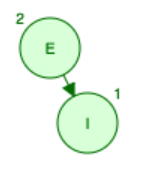
\includegraphics[scale=0.4]{em}
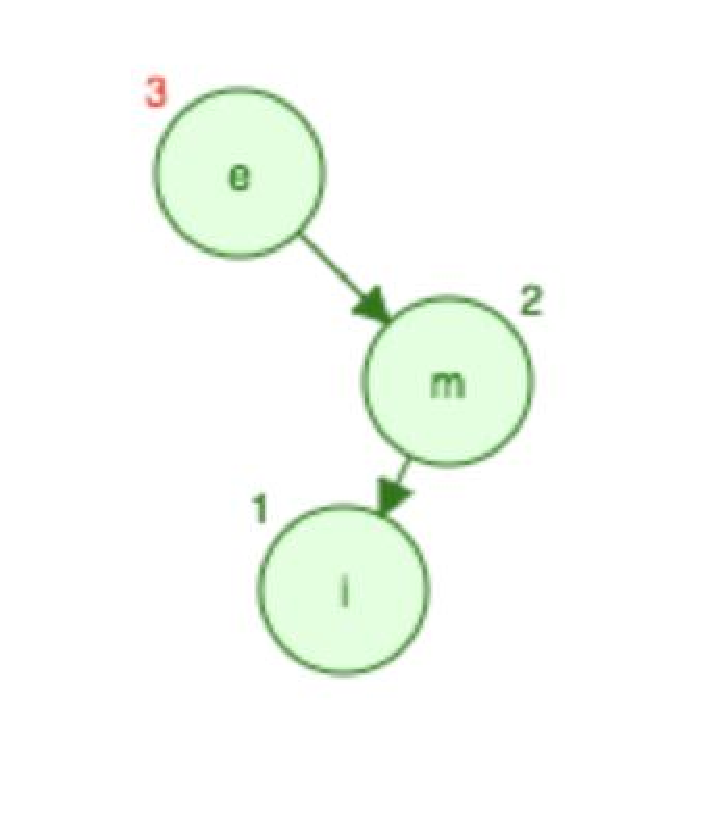
\includegraphics[scale=0.4]{emiBefore}
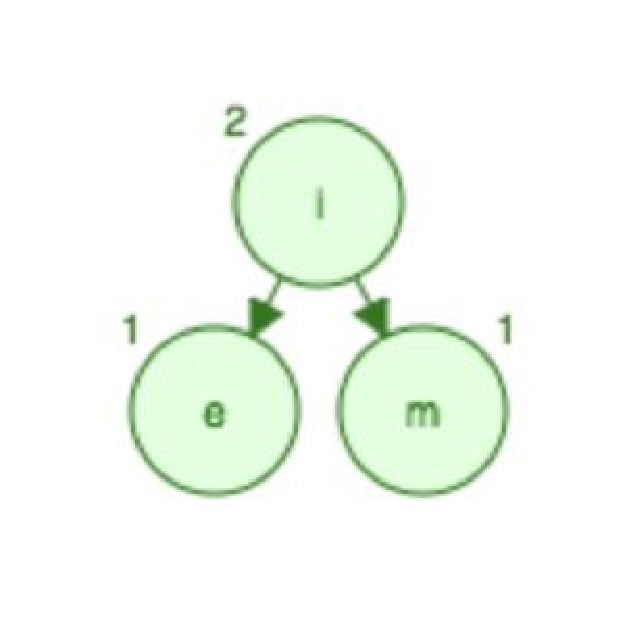
\includegraphics[scale=0.5]{emiAfter}

Enkelrotationer är den mindre komplexa rotationssorten för AVL-träd. När en en nod har subträd som vars djup skiljer sig med mer än ett behövs det balanseras upp vilket är rotationernas jobb. För att börja med ett simpelt exempel så har vi använt oss av bokstäverna $E, I $ och $M$. Vi börjar med att lägga till roten i det binära sökträdet, i det här fallet är det ett $E$, därefter lägger vi till ett $I$ som är större än $E$ och läggs därför till höger i ett subträd till roten. Om vi sen ska lägga till ett $M$ till trädet så är det större än båda noderna som tidigare lagts till vilket betyder att $M$'et läggs till som ett barn till noden $I$. När kontrollen sen sker om balansen upprätthålls så börjar kontrollen i den noden som senast lades till, kontrollen förflyttas till föräldern till den tidigare noden och upptäcker att det högra subträdet har djupet 1 medans det vänsta har djupet 0 vilket är fullt tillåtet då skillnaden inte får vara större än 1. När kontrollen sen kommer upp till roten så kontrolleras subträden och skillnaden är då mer än 1, närmare bestämt är djupet på vänstra subträdet 0 och högra 2. För att åtgärda balansen i trädet så flyttas noden till höger om roten, i detta fall $I$, ett steg åt vänster. Den tidigare roten är nu en barnnod till noden som tidigare låg som ett barn i höger subträd. Enkelrotationen har löst balansen med ett steg där obalansen låg i roten. 

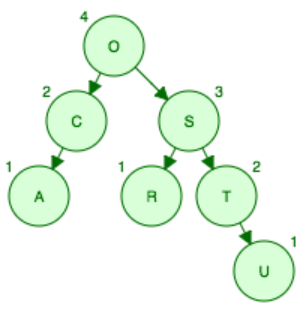
\includegraphics[scale=0.3]{advEnk}
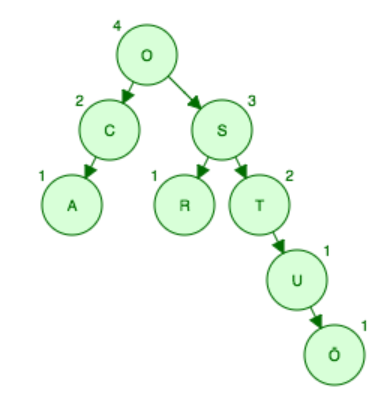
\includegraphics[scale=0.3]{advEnkB}
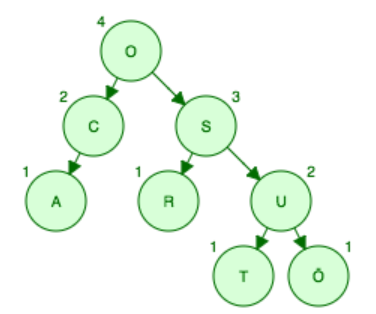
\includegraphics[scale=0.3]{advEnkA}

Enkelrotationer är dock något som inte bara används av rotnoden i trädet utan kan användas av noter som ligger längre ner också. Nästa exempel visar när en enkelrotation sker på ett annat djup än rotens djup. I den första bilden ovanför detta stycke så har vi ett träd av bokstäverna \textit{O-S-C-A-R-T-U}. Den andra bilden visar hur ett \textit{Ö} läggs till i trädet. När \textit{Ö} läggs till jämförs den först med rotnoden som  är $O$, eftersom \textit{Ö} är större så flyttas den ner till höger, \textit{Ö} är också större än $S$ som är barnnod till $O$ och kommer därför flyttas ner yttligare ett steg till höger, där stöter den sedan på ett $T$ som är barnnod till $S$, \textit{Ö}är större och flyttas ner till höger, samma sak händer där när \textit{Ö} stöter på $U$, och flyttas ner till höger. När balansen kontrolleras så uppstår det en obalans redan vid $T$-noden. Där är det återigen en skillnad som är större än 1 mellan det högra subträdet och det vänstra, vilket då behöver balanseras med hjälp av enkelrotationen. Sista bilden visar att $U$ flyttar upp ett steg, $T$ läggs som vänstra barnet till $U$ då $T < U$ och \textit{Ö} hänger bara på när $U$ flyttas upp. 

\section*{Dubbelrotationer}

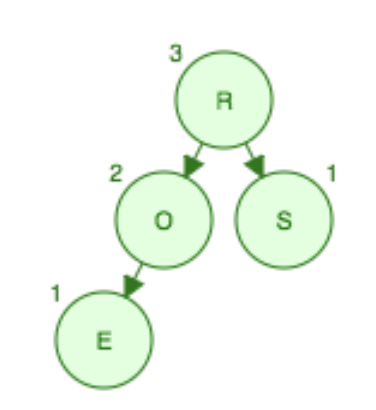
\includegraphics[scale=0.5]{Dub1}
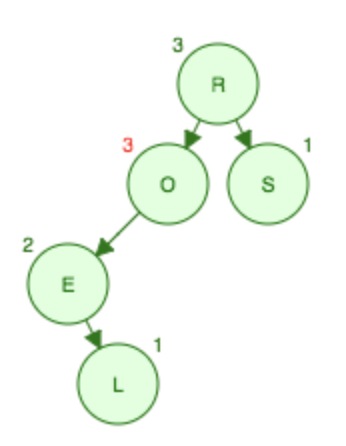
\includegraphics[scale=0.5]{Dub2}
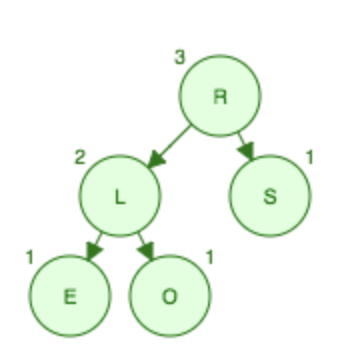
\includegraphics[scale=0.5]{Dub3}

Enkelrotationer räcker långt men i vissa fall så krävs det att en dubbelrotation används istället. För att förklara hur dubbelrotationer används och varför det behövs har vi använt oss av ett enkelt träd där vi lagt in värdena \textit{R-O-S-E}. Om vi skulle lägga in ett värde som är mindre än $E$ så hade det endast krävs en enkelrotation åt höger vid noden $O$ då det blir obalans där. Men om vi istället skulle lägga in ett värde som är mindre än $O$ men större än $E$, då skulle en enkelrotation vid $E$ endast bidra till att sökträdet blir felaktigt då vänsterbarnet till $E$ hade varit  större, vilket inte riktigt är det vi är ute efter. Som exemplet visar så läggs värdet $L$ in i sökträdet och det placeras så att det bildas en obalans i $O$-noden, därav krävs en balansering. För att det ska bli rätt djup men också korrekt uppdelning av noderna så flyttas den senaste noden, $L$ upp och dess vänsterbarn blir $E$ och högerbarnet blir noden $O$ som det tidigare var en obalans i. Då ser vi att $L < O$ och  $L > E$ vilket är korrekt och dubbelrotationen har gjort sitt jobb.

Enkelrotationer skiljer sig från dubbelrotationer på så vis att om det nya värdet som läggs in är större än sin förälder, så är noden som obalansen sker i mindre än både sitt barn som det nya värdet är barn till och det nya värdet. Det går alltså att lyfta barnet ett steg upp det alltid kommer vara ett värde emellan det nya värdet och sin förälder, föräldern bli naturligt vänsterbarn till den uppflyttade noden och högerbarnet är som tidigare det senast inlagda värdet. 
Dubbelrotation behövs alltså när värdena inte kan flyttas med ett steg, utan det krävs en rotation följt av en annan för att flytta värdena rätt och fortfarande bibehålla ordningen så att alla noder landar på rätt plats. Bilderna nedan visar problemet som tagits upp att trädet inte blir korrekt om en enkelrotation skulle tillämpas. 

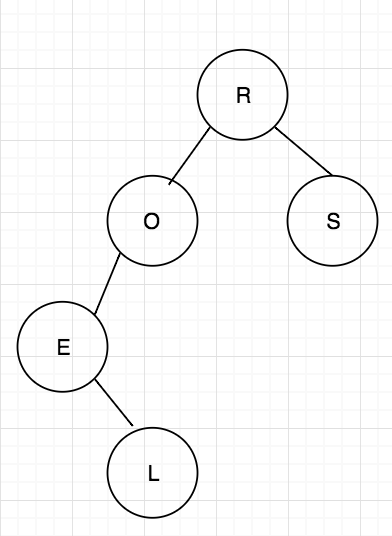
\includegraphics[scale=0.4]{enkelRot} 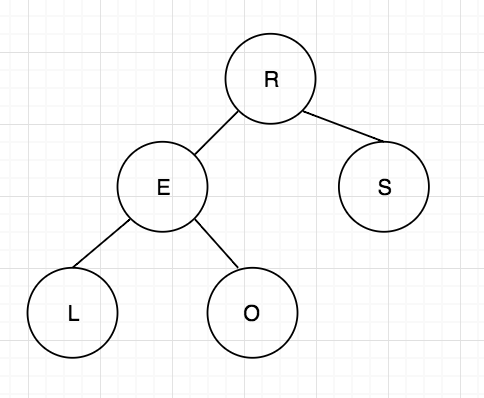
\includegraphics[scale=0.4]{enkelRot1}
\end{document}
